%!TEX encoding = UTF-8 Unicode
% $Id: 20-continuations.tex 18 2014-03-12 22:35:24Z binghe $

\chapter{\continuation{}~(continuation)}
\label{chap:continuations}
\index{continuations \continuation{}s}

\continuation{}是在运行中被暂停了的程序:即含有计算状态的单个函数型对象。
当这个对象被求值时,就会在它上次停下来的地方重新启动之前保存下来的计算。对于求解特定类型的问
题,能够保存程序的状态并在之后重启是非常有用的。例如在多进程中,
\continuation{}可以很方便地表示挂起的进程。而在非确定性的搜索问题
里,\continuation{}可以用来表示搜索树中的节点。

要一下子理解\continuation{}或许会有些困难。本章分两步来探讨这个主题。本
章的第一部分会先分析\continuation{}在~Scheme\note{258} 中的应用,这门语言内置了对\continuation{}
的支持。一旦说清楚了\continuation{}的行为,第二部分将展示如
何使用宏在~Common Lisp 程序里实现\continuation{}。
第~\ref{chap:multiple_processes}--\ref{chap:prolog} 章都将用到这里定义
的宏。

\section{Scheme \continuation{}}
\label{sec:scheme_continuations}

Scheme 和~Common Lisp 在几个主要方面存在着不同,其中之一就是:前者拥有显式的
\continuation{}支持。本节展示的是\continuation{}在~Scheme 中的工作方式。
(图~\ref{fig:some_differences_between_scheme_and_common_lisp} 列出
了~Scheme 和~Common Lisp 间一些其他的区别。)

\begin{figure}
  \begin{enumerate}
  \item 在~Common Lisp 眼中,一个符号的~\texttt{symbol-value}
    和~\texttt{symbol-function} 是不一样的,而~Scheme 对两者不作区分。在~Scheme 里面,
    变量只有唯一对应的值,它可以是个函数,也可以是另一种对象。因此,在~Scheme 中就不
    需要~\sq~或者~\texttt{funcall} 了。Common Lisp 的:
\begin{lstlisting}
(let ((f #'(lambda (x) (1+ x))))
  (funcall f 2))
\end{lstlisting}
    在~Scheme 中将变成:
\begin{lstlisting}
(let ((f (lambda (x) (1+ x))))
  (f 2))
\end{lstlisting}
  \item 由于~Scheme 只有一个名字空间\index{name-spaces},因而它没有必要为各个名字空间专门设置对应的赋值
    操作符~(例如~\texttt{defun} 和~\texttt{setq})。取而代之,它使用~\texttt{define},
    \verb|define| 的作用和~\verb|defvar| 大致相当,同时用~\texttt{set!} 替代
    了~\texttt{setq}。在用~\texttt{set!} 为全局变量赋值前,必须先用~\texttt{define} 创建这个变量。
  \item 在~Scheme 中,通常用~\texttt{define} 定义有名函数,它行使着
    ~\texttt{defun} 和~\texttt{defvar} 在~Common Lisp 中的功能。Common Lisp 的:
\begin{lstlisting}
(defun foo (x) (1+ x))
\end{lstlisting}
    有两种可能的~Scheme 翻译:
\begin{lstlisting}
(define foo (lambda (x) (1+ x)))
(define (foo x) (1+ x))
\end{lstlisting}
  \item 在~Common Lisp 中,函数的参数按从左到右的顺序求值。而在~Scheme 中,
    有意地不对求值顺序加以规定。\index{evaluation!order of!in Scheme}(并且语言的实现者对于忘记这点的人幸灾乐祸。)
  \item Scheme 不用~\verb|t| 和~\verb|nil|,相应的,它有~\verb|#t|
    和~\verb|#f|。空列表,\verb|()|,在某些实现里为真,而在另一些实
    现里为假。
  \item \texttt{cond} 和~\texttt{case} 表达式里的默认子句在~Scheme 中
    带有~\texttt{else} 关键字,而不是~Common Lisp 中的~\texttt{t}。
  \item 某些内置操作符的名字被改掉了:\texttt{consp} 成了~\texttt{pair?},
    而~\texttt{null} 则是~\texttt{null?},\texttt{mapcar} (几乎)
    是~\texttt{map},等等。通常根据上下文,应该能看出这些操作符的意思。
  \end{enumerate}
  \caption{Scheme 和~Common Lisp 之间的一些区别}
  \label{fig:some_differences_between_scheme_and_common_lisp}
  \index{Scheme!vs. Common Lisp}
  \index{Common Lisp!vs. Scheme}
\end{figure}

\continuation{}是一个代表着计算的将来的函数。不管是哪一个表达式被求值,
总会有谁在翘首以待它将要返回的值。例如,在
\begin{lstlisting}
(/ (- x 1) 2)
\end{lstlisting}
中,当求值~\verb|(- x 1)| 时,外面的~\verb|/| 表达式就在等着这个
值,同时,还有另外一个式子也在等着\emph{它的}值,依此类推下去,最后总是回
到~toplevel 上\pozhehao{}\verb|print| 正等在那里。

无论何时,我们都可以把\continuation{}视为带一个参数的函数。如果上
面的表达式被输入到~toplevel,那么当子表达式~\verb|(- x 1)| 被求值时,
\continuation{} 将是:
\begin{lstlisting}
(lambda (val) (/ val 2))
\end{lstlisting}
也就是说,接下来的计算可以通过在返回值上调用这个函数来重现。如果该表达式
在下面的上下文中出现
\begin{lstlisting}
(define (f1 w)
  (let ((y (f2 w)))
    (if (integer? y) (list 'a y) 'b)))

(define (f2 x)
  (/ (- x 1) 2))
\end{lstlisting}
并且~\texttt{f1} 在~toplevel 下被调用,那么当~\texttt{(- x 1)} 被求值
时,\continuation{}将等价于
\begin{lstlisting}
(lambda (val)
  (let ((y (/ val 2)))
    (if (integer? y) (list 'a y) 'b)))
\end{lstlisting}

在~Scheme 中,\continuation{} 和函数同样是第一类对象。你可以要求~Scheme
返回当前的\continuation{},然后它将为你生成一个只有单个参数的函数,以表示未
来的计算。你可以任意长时间地保存这个对象,然后在你调用它时,它将重启当
它被创建时所发生的计算。

\continuation{}可以理解成是一种广义的闭包。闭包就是一个函数加上一些指向
闭包创建时可见的词法变量的指针。\continuation{}则是一个函数加上一个
指向其创建时所在的整个栈\index{stacks 栈!in continuations}的指针。当\continuation{}被求值时,它返回
的是使用自己的栈拷贝算出的结果,而没有用当前栈。如果某个\continuation{}是在~$T_1$
时刻创建的,而在~$T_2$ 时刻被求值,那么它求值时使用的将是~$T_1$ 时刻的栈。

Scheme 程序通过内置操作符~\verb|call-with-current-continuation| (缩写为
~\verb|call/cc|)
\index{call-with-current-continuation (call/cc)@\texttt{call-with-current-continuation} (\texttt{call/cc})} 
来访问当前\continuation{}。当一个程序在
一个单个参数的函数上调用~\texttt{call/cc} 时:
\begin{lstlisting}
(call-with-current-continuation
  (lambda (cc)
    ...))
\end{lstlisting}
这个函数将被传进另一个代表当前\continuation{}的函数。通过将~\texttt{cc}
的值存放在某个地方,我们就可以保存在~\texttt{call/cc} 那一点上的计算状
态。

在这个例子里,我们~\texttt{append} 出一个列表,列表的最后一个元素是一
个~\texttt{call/cc} 表达式的返回值:
\begin{lstlisting}
> (define frozen)
FROZEN
> (append '(the call/cc returned)
          (list (call-with-current-continuation
                  (lambda (cc)
                    (set! frozen cc)
                    'a))))
(THE CALL/CC RETURNED A)
\end{lstlisting}
这个~\texttt{call/cc} 返回了~\texttt{a},但它首先将\continuation{}保存在
了全局变量~\texttt{frozen} 中。

调用~\texttt{frozen} 会导致在~\texttt{call/cc} 那一点上的旧的计算重新开始。无
论我们传给~\texttt{frozen} 什么值,这个值都将作为~\texttt{call/cc} 的值返回:
\begin{lstlisting}
> (frozen 'again)
(THE CALL/CC RETURNED AGAIN)
\end{lstlisting}
\continuation{}不会因为被求值而用完。它们可以被重复调用,就像任何其他的
函数型对象一样:
\begin{lstlisting}
> (frozen 'thrice)
(THE CALL/CC RETURNED THRICE)
\end{lstlisting}

当我们在某些其他的计算里调用一个\continuation{}时,我们可以更清楚地看到
所谓返回到原先的栈\index{stacks 栈!in continuations}上是什么意思:
\begin{lstlisting}
> (+ 1 (frozen 'safely))
(THE CALL/CC RETURNED SAFELY)
\end{lstlisting}
这里,紧接着的~\texttt{+} 当~\texttt{frozen} 调用时被忽略掉了。后者返
回到了它首次被创建时的栈上:先经过~\texttt{list},然后
是~\texttt{append},直到~toplevel。如果~\texttt{frozen} 像正常函数调用
那样返回了一个值,那么上面的表达式将在试图给一个列表加~1 时产生一个错
误。

各\continuation{}并不会每人都分到自己的一份栈的拷贝\label{share-between-continuations}。它们可能跟其他\continuation{}或者当
前正在进行的计算共享一些变量。在下面这个例子里,两个\continuation{}共享
了同一个栈:
\begin{lstlisting}
> (define froz1)
FROZ1
> (define froz2)
FROZ2
> (let ((x 0))
    (call-with-current-continuation
      (lambda (cc)
        (set! froz1 cc)
        (set! froz2 cc)))
    (set! x (1+ x))
    x)
1
\end{lstlisting}
因此调用任何一个都将返回后继的整数:
\begin{lstlisting}
> (froz2 ())
2
> (froz1 ())
3
\end{lstlisting}
由于~\texttt{call/cc} 表达式的值将被丢弃,所以无论我们给~\texttt{froz1}
和~\texttt{froz2} 什么参数都无关紧要。

现在能保存计算的状态了,我们可以用它做什么呢?
第~\ref{chap:multiple_processes}--\ref{chap:prolog} 章致力于使用
\continuation{}的应用。这里将要考察一个比较简单的例子,它能够体现出使用保存状态编程的特色:
假设有一组树,我们想从每棵树都取出一个元素,组成一个列表,直到获得一个满足某种条件的组合。

\begin{figure}
\centering
  \subfigure[\texttt{t1}]{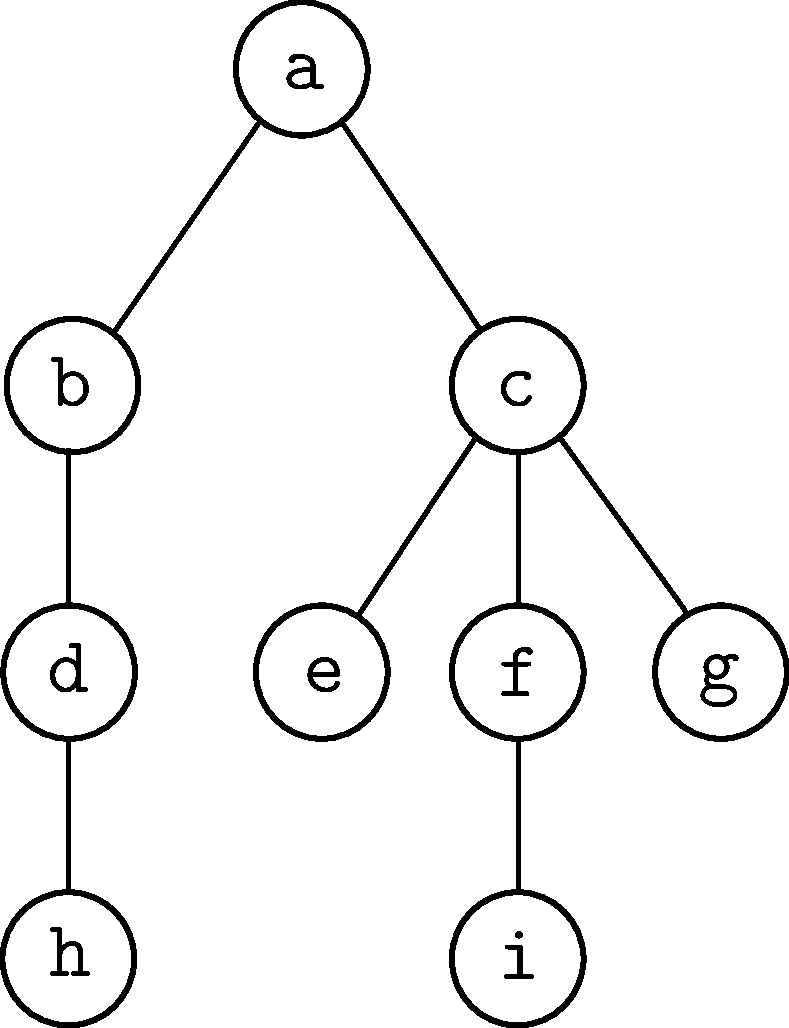
\includegraphics[width=0.25\textwidth]{two-trees-1.pdf}}
  \hspace{0.1\textwidth}
  \subfigure[\texttt{t2}]{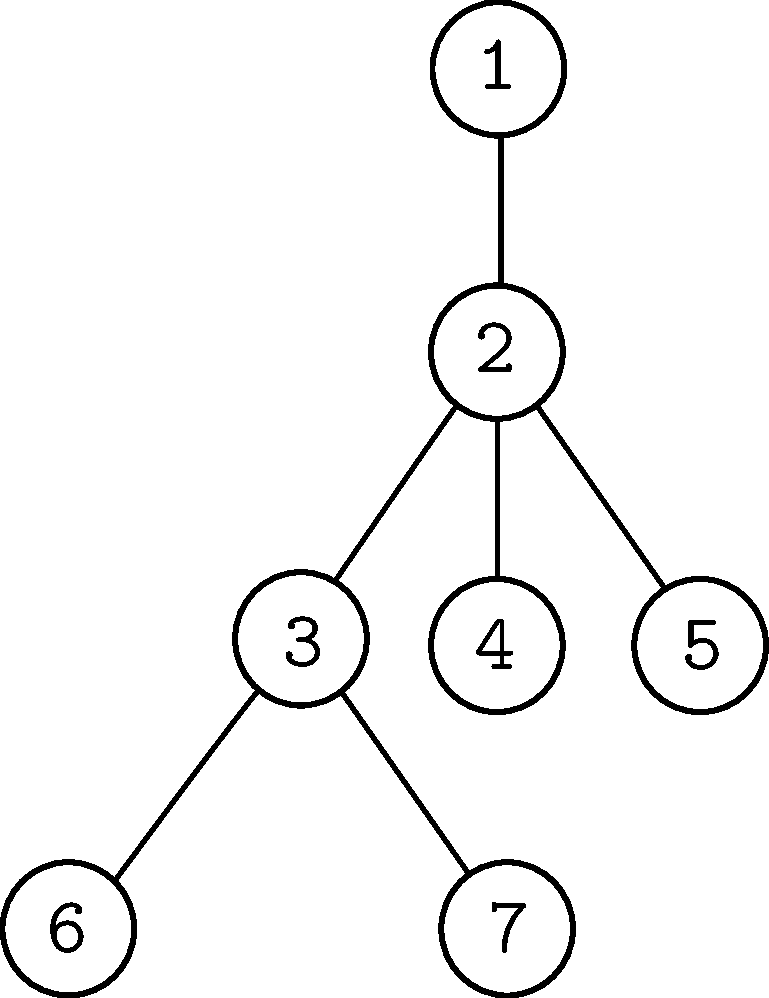
\includegraphics[width=0.25\textwidth]{two-trees-2.pdf}}
  \caption{两棵树}
  \label{fig:two_trees}
\end{figure}

树可以用嵌套列表来表示\index{lists!as trees}。第~\pageref{sec:function:recursion_on_subtrees}
页上描述了一种将一类树表示成列表的方法。这里我们采用另一种方法,允许内
部节点带有~(原子的) 值,以及任意数量的孩子。在这种表示方法里,内部节点
变成了一个列表;其~car 包含保存在这个节点上的值,其~cdr 包含该节点孩子
的表示。例如,图~\ref{fig:two_trees} 里显示的两棵树可以被表示成:
\begin{lstlisting}
(define t1 '(a (b (d h)) (c e (f i) g)))
(define t2 '(1 (2 (3 6 7) 4 5)))
\end{lstlisting}

\begin{figure}
\begin{lstlisting}
(define (dft tree)
  (cond ((null? tree) ())
        ((not (pair? tree)) (write tree))
        (else (dft (car tree))
              (dft (cdr tree)))))

(define *saved* ())

(define (dft-node tree)
  (cond ((null? tree) (restart))
        ((not (pair? tree)) tree)
        (else (call-with-current-continuation
                (lambda (cc)
                  (set! *saved*
                        (cons (lambda ()
                                (cc (dft-node (cdr tree))))
                              *saved*))
                  (dft-node (car tree)))))))

(define (restart)
  (if (null? *saved*)
      'done
      (let ((cont (car *saved*)))
        (set! *saved* (cdr *saved*))
        (cont))))

(define (dft2 tree)
  (set! *saved* ())
  (let ((node (dft-node tree)))
    (cond ((eq? node 'done) ())
          (else (write node)
                (restart)))))
\end{lstlisting}
  \caption{用\continuation{}来遍历树}
  \label{fig:tree_traversal_using_continuations}
  \index{stacks 栈!use for iteration}
\end{figure}

图~\ref{fig:tree_traversal_using_continuations} 中的函数能在这样的树上做深
度优先搜索。在实际的程序里,我们可能想要在遇到节点时用它们做一些事。
这里只是打印它们。为了便于比较,这里给出的函数~\texttt{dft} 
实现了通常的深度优先遍历:
\begin{lstlisting}
> (dft t1)
ABDHCEFIG()
\end{lstlisting}
函数~\texttt{dft-node} 按照同样的路径遍历这棵树,但每次只处理一个节点。
当~\texttt{dft-node} 到达一个节点时,它跟着节点的~car 走,并且
在~\texttt{*saved*} 里压入一个\continuation{}来浏览其~cdr 部分。
\begin{lstlisting}
> (dft-node t1)
A
\end{lstlisting}
调用~\texttt{restart} 可以继续遍历,作法是弹出最近保存的
\continuation{}并调用它。
\begin{lstlisting}
> (restart)
B
\end{lstlisting}
最后,所有之前保存的状态都用完了,\texttt{restart} 通过返回~\texttt{done}
来通告这一事实:
\begin{lstlisting}
$\vdots$
> (restart)
G
> (restart)
DONE
\end{lstlisting}

最后,函数~\texttt{dft2} 把我们刚刚手工完成的工作干净漂亮地一笔带过:
\begin{lstlisting}
> (dft2 t1)
ABDHCEFIG()
\end{lstlisting}
注意到在~\texttt{dft2} 的定义里没有显式的递归或迭代\index{iteration!without loops}:后继的节点被打印
出来,是因为由~\texttt{restart} 引入的\continuation{}总是返回
到~\texttt{dft-node} 中同样的~\texttt{cond} 子句那里。

这种程序的工作方式就跟采矿\index{mines 采矿}差不多。它先调用~\texttt{dft-node} 初步挖出一
个矿坑。一旦返回值不是~\texttt{done},\texttt{dft-node} 后面的代码
将调用~\texttt{restart} 将控制权发回到栈上。这个过程会一直持续,直到到返回值表明矿
被采空。这时,\texttt{dft2} 将不再打印返回值,而是返回~\verb|#f|。
使用\continuation{}的搜索方式带来了一种编写程序的新思路:将合适
的代码放在栈上,然后不断地返回到那里来获得结果。

如果我们只是想同时遍历一棵树,就像~\texttt{dft2} 里那样,那么实在没
有必要使用这种技术。\texttt{dft-node} 的优势在于,可以同时运行它的多个
实例。假设有\emph{两}棵树,并且我们想要以深度优先的顺序生成其中
元素的叉积\index{trees 树!cross-products of 叉积}。
\begin{lstlisting}
> (set! *saved* ())
()
> (let ((node1 (dft-node t1)))
    (if (eq? node1 'done)
        'done
        (list node1 (dft-node t2))))
(A 1)
> (restart)
(A 2)
$\vdots$
> (restart)
(B 1)
$\vdots$
\end{lstlisting}
借助常规技术,我们必须采取显式的措施来保存我们在两棵树中的位置。而通
过\continuation{},则能非常自然地维护两个正在进行的遍历操作的状态。对于诸如本例的
简单情形,要保存我们在树中的位置还不算太难。树是持久性的数据结构,所以我
们至少有办法找到~``我们在树中的位置''。\continuation{}的过人之处在于,
即使没有持久性的数据结构与之关联,它同样可以在\emph{任何}的计算过程中轻松保存我们的位置。
这一计算甚至也不需要具有有限数量的状态,只要重启它们有限次就行了。

正如第~\ref{chap:prolog} 章将要展示的,这两种考虑被证实在~Prolog 的
实现中至关重要。在~Prolog 程序里,“搜索树”\index{search trees}并非真正的数据结构,而
只是程序生成结果的一种隐式方式。而且这些树经常是无穷大的,这种情况下,我
们不能指望在搜索下一棵树之前把整棵树都搜完,所以只得想个办法保存我们的位置,
除此之外别无选择。

\section{\continuation{}传递宏}
\label{sec:continuation-passing_macros}
\index{continuation-passing macros}

虽然~Common Lisp 没有提供~\texttt{call/cc},但是再加把劲,我们就可以
像在~Scheme 里那样做到同样的事情了。本节展示如何用宏在~Common Lisp 程序
中构造\continuation{}。Scheme 的\continuation{}给了我们两样东西:
\begin{enumerate}
\item \continuation{}被创建时所有变量的绑定。
\item 计算的状态\pozhehao{}从那时起将要发生什么。
\end{enumerate}
在一个词法作用域的~Lisp 里,闭包给了我们前者。可以看出我
们也能使用闭包来获得后者,办法是把计算的状态同样也保存在变量绑定里。

%% Figure 20.4: change global value of *cont* according to errata
\begin{figure}
\begin{lstlisting}
(defvar *actual-cont* #'values)

(define-symbol-macro *cont*
  *actual-cont*)

(defmacro =lambda (parms &body body)
  `#'(lambda (*cont* ,@parms) ,@body))

(defmacro =defun (name parms &body body)
  (let ((f (intern (concatenate 'string
                                "=" (symbol-name name)))))
    `(progn
       (defmacro ,name ,parms
         `(,',f *cont* ,,@parms))
       (defun ,f (*cont* ,@parms) ,@body))))

(defmacro =bind (parms expr &body body)
  `(let ((*cont* #'(lambda ,parms ,@body))) ,expr))

(defmacro =values (&rest retvals)
  `(funcall *cont* ,@retvals))

(defmacro =funcall (fn &rest args)
  `(funcall ,fn *cont* ,@args))

(defmacro =apply (fn &rest args)
  `(apply ,fn *cont* ,@args))
\end{lstlisting}
  \caption{\continuation{}传递宏}
  \label{fig:continuation-passing_macros}
  \index{lambda@\texttt{=lambda}}
  \index{defun@\texttt{=defun}}
  \index{bind@\texttt{=bind}}
  \index{values@\texttt{=values}}
  \index{funcall@\texttt{=funcall}}
  \index{apply@\texttt{=apply}}
\end{figure}

图~\ref{fig:continuation-passing_macros} 给出的宏让我们能在保
留\continuation{}的情况下,进行函数调用。\index{functions 函数!combined with macros}这些宏取代了几个内置的~Common
Lisp form,它们被用来定义函数,进行函数调用,以及返回函数值。

如果有函数需要使用\continuation{},或者这个函数所调用的函数要用到\continuation{},那么该函数
就该用~\texttt{=defun} 而不是~\texttt{defun} 定义\note{266}。
\texttt{=defun} 的语法和~\texttt{defun} 相同,但其效果有些微妙的差别。
\texttt{=defun} 定义的并不是单单一个函数,它实际上定义了一个函数和一个宏,这个宏会展开
成对该函数的调用\index{macros 宏!macro-defining}\index{macros 宏!combined with functions}。
(宏定义必须在先\index{macros 宏!position in source code},原因是被定义的函数有可能会调用自己。)
函数的主体就是传给~\texttt{=defun} 的那个,但还另有一个形参,
即~\verb|*cont*|\index{*cont*@\texttt{*cont*}},它被连接在原有的形参列表上。在宏展开式里,\texttt{*cont*} 会和其他参数一同传给
这个函数。所以
\begin{lstlisting}
(=defun add1 (x) (=values (1+ x)))
\end{lstlisting}
宏展开成
\begin{lstlisting}
(progn (defmacro add1 (x)
         `(=add1 *cont* ,x))
       (defun =add1 (*cont* x)
         (=values (1+ x))))
\end{lstlisting}

当调用~\texttt{add1} 时,实际被调用的不是函数而是个宏。这个宏
会展开成一个函数调用%
\footnote{由~\texttt{=defun} 产生的函数被有意地赋予了~intern\index{intern@\texttt{intern}} 了的名字,好让这些函数能够被~
  \texttt{trace}\index{trace@\texttt{trace}}。如果没有必要做~trace 的话,用 gensym 来作为它们的名字应该会更安全些。}\label{trace}%
,但是另外带了一个参数:\texttt{*cont*}。所以,在调用~\texttt{=defun} 定义的操作符的时候,
\texttt{*cont*} 的当前值总是被默默地传递着。

那~\texttt{*cont*} 有什么用呢?它将被绑定到当前的\continuation{}。
\texttt{=values} 的定义显示了这个\continuation{}的用场。只要是用
~\texttt{=defun} 定义的函数,都必须通过~\texttt{=values} 来返回值,或者
调用另一个使用~\verb|=values| 的函数。\texttt{=values} 的语法与~Common Lisp
的~\texttt{values} 相同。如果有个带有相同数量参数的~\texttt{=bind}\label{page:bind} 等着它的话,
它可以返回多值,但它不能返回多值到~toplevel。\note{267}

参数~\texttt{*cont*} 告诉那个由~\texttt{=defun} 定义的函数对其返回值做
什么。当~\texttt{=values} 被宏展开时,它将捕捉~\texttt{*cont*}\index{capture 捕捉!intentional},并用
它模拟从函数返回值的过程。表达式
\begin{lstlisting}
(=values (1+ n))
\end{lstlisting}
会展开成
\begin{lstlisting}
(funcall *cont* (1+ n))
\end{lstlisting}
在~toplevel 下,\texttt{*cont*} 的值是~\verb|#'values|\footnote{译
  者注:原文是~``\texttt{*cont*} 的值是~\texttt{identity}'',这是错误
  的。并且原书勘误修正了图~\ref{fig:continuation-passing_macros}
  中对应的~\texttt{*cont*} 定义,这里译文也随之做了修改。},
这就相当于一个真正的~\texttt{values} 多值返回。当我们在~toplevel
下调用~\texttt{(add1 2)} 时,这个调用的宏展开式与下式等价
\begin{lstlisting}
(funcall #'(lambda (*cont* n) (=values (1+ n))) *cont* 2)
\end{lstlisting}
\texttt{*cont*} 的引用在这种情况下将得到全局绑定。因而,\texttt{=values} 表
达式在宏展开后将等价于下式
\begin{lstlisting}
(funcall #'values (1+ n))
\end{lstlisting}
即把在~\texttt{n} 上加~\texttt{1},并返回结果。

在类似~\texttt{add1} 的函数里,我们克服了重重困难,不过是
为了模拟~Lisp 进行函数调用和返回值的过程:
\begin{lstlisting}
> (=defun bar (x)
    (=values (list 'a (add1 x))))
BAR
> (bar 5)
(A 6)
\end{lstlisting}
关键在于,现在有了``函数调用''和``函数返回''可供差遣,而且如果
愿意的话,我们还可以把它们用在其他地方。

我们之所以能获得\continuation{}的效果,要归功于对~\texttt{*cont*} 的操控。虽
然~\texttt{*cont*} 的值是全局的,但这个全局变量很少用到:
\texttt{*cont*} 几乎总是一个形参,它被~\texttt{=values} 以及
用~\texttt{=defun} 定义的宏所捕捉。例如在~\texttt{add1} 的函数体里,
\texttt{*cont*} 就是一个形参而非全局变量\index{variables 变量!global 全局}。这个区别是很重要的,因为如
果~\texttt{*cont*} 不是一个局部变量的话这些宏将无法工作。\footnote{译
  者注:原书中在这里还有一句话:``That's why \texttt{*cont*} is given
  its initial value in a \texttt{setq} instead of a \texttt{defvar}:
  the latter would also proclaim it to be \texttt{special}.'' 
  原作者假设~\texttt{*cont*} 全局变量是词法作用域的,但这违
  反了~Common Lisp 标准。为了能在现代~Common Lisp 实现上运行这些代码,
  译文采纳了~\href{http://www.cliki.net/On\%20Lisp}{\textsc{Cliki}} 上
  给出的一个解决方案,使用符号宏来模拟词法变量。具体参见
  图~\ref{fig:continuation-passing_macros} 中修改过的代码。}
图~\ref{fig:continuation-passing_macros} 中的第三个宏,\texttt{=bind},
其用法和~\texttt{multiple-value-bind} 相同。它接受一个参
数列表,一个表达式,以及一个代码体:参数将被绑定到表达式返回的值上,而
代码体在这些绑定下被求值。倘若一个由~\texttt{=defun} 定义的函数,
在被调用之后,需要对另一个表达式进行求值,那么就应该使用~\texttt{=bind} 宏。
\begin{lstlisting}
> (=defun message ()
    (=values 'hello 'there))
MESSAGE
> (=defun baz ()
    (=bind (m n) (message)
      (=values (list m n))))
BAZ
> (baz)
(HELLO THERE)
\end{lstlisting}
注意到~\texttt{=bind} 的展开式会创建一个称为~\texttt{*cont*} 的新
变量。\texttt{baz} 的主体展开成:
\begin{lstlisting}
(let ((*cont* #'(lambda (m n)
                  (=values (list m n)))))
  (message))
\end{lstlisting}
然后会变成:
\begin{lstlisting}
(let ((*cont* #'(lambda (m n)
                  (funcall *cont* (list m n)))))
  (=message *cont*))
\end{lstlisting}
由于~\texttt{*cont*} 的新值是~\texttt{=bind} 表达式的代码体,所以
当~\texttt{message} 通过函数调用~\texttt{*cont*} 来~``返回'' 时,结果
将是去求值这个代码体。尽管如此~(并且这里是关键),在~\texttt{=bind} 的
主体里:
\begin{lstlisting}
#'(lambda (m n)
    (funcall *cont* (list m n)))
\end{lstlisting}
作为参数传递给~\texttt{=baz} 的~\texttt{*cont*} 仍然是可见的,所以当代
码的主体求值到一个~\texttt{=values} 时,\emph{它}将能够返回到最初的
主调函数那里。所有闭包环环相扣:每个~\texttt{*cont*} 的绑定
都包含了上一个~\texttt{*cont*} 绑定的闭包,它们串成一条锁链\index{chains of closures},锁链的尽头指向
那个全局的值。

在这里,我们也可以观察到更小规模的同样现象:
\begin{lstlisting}
> (let ((f #'values))
    (let ((g #'(lambda (x) (funcall f (list 'a x)))))
      #'(lambda (x) (funcall g (list 'b x)))))
#<Interpreted-Function BF6326>
> (funcall * 2)
(A (B 2))
\end{lstlisting}
本例创建了一个函数,它是含有指向~\texttt{g} 的引用的闭包,
而~\texttt{g} 本身也是一个含有到~\texttt{f} 的引用的闭包。第~\pageref{fig:compilation_with_static_reference} 页上的网络编
译器中曾构造过类似的闭包链。

剩下两个宏,分别是~\texttt{=apply} 和~\texttt{=funcall},它们适用于
由~\texttt{=lambda} 定义的函数。注意那些用~\texttt{=defun} 定义出来
的~``函数'',因为它们的真实身份是宏,所以不能作为参数传给~\texttt{apply}
或~\texttt{funcall}。解决这个问题的方法类似于第~\pageref{the_cons_4}
页上提到的技巧。也就是把调用包装在另一个~\texttt{=lambda} 里面:
\begin{lstlisting}
> (=defun add1 (x)
    (=values (1+ x)))
ADD1
> (let ((fn (=lambda (n) (add1 n))))
    (=bind (y) (=funcall fn 9)
      (format nil "9 + 1 = ~A" y)))
"9 + 1 = 10"
\end{lstlisting}

\begin{figure}
  \begin{enumerate}
  \item 一个用~\texttt{=defun} 定义的函数的参数列表必须完全由参数名组
    成。
  \item 使用\continuation{},或者调用其他做这件事的函数的函数,必须
    用~\texttt{=lambda} 或~\texttt{=defun} 来定义。
  \item 这些函数必须终结于用~\texttt{=values} 来返回值,或者调用其他遵守
    该约束的函数。
  \item\label{itm:tail-call} 如果一个~\texttt{=bind},\texttt{=values},或
    者~\texttt{=funcall} 表达式出现在一段代码里,它必须是一个尾调用。
    任何在~\texttt{=bind} 之后求值的代码必须放在其代码体里。所以如果我
    们想要依次有几个~\texttt{=bind},它们必须被嵌套:
\begin{lstlisting}
(=defun foo (x)
  (=bind (y) (bar x)
    (format t "Ho ")
    (=bind (z) (baz x)
      (format t "Hum.")
      (=values x y z))))
\end{lstlisting}
  \end{enumerate}
  \caption{\continuation{}传递宏的限制}
  \label{fig:restrictions_on_continuation-passing_macros}
  \index{continuation-passing macros!restrictions on}
\end{figure}

图~\ref{fig:restrictions_on_continuation-passing_macros} 总结了所有因
\continuation{}传递宏而引入的限制。如果有函数既不保存\continuation{},也不调用其他保存\continuation{}的函数,
那它就没有必要使用这些特殊的宏。比如像~\texttt{list} 这样的内置函数就没有这个需要。

\begin{figure}
\begin{lstlisting}
(defun dft (tree)
  (cond ((null tree) nil)
        ((atom tree) (princ tree))
        (t (dft (car tree))
           (dft (cdr tree)))))

(defvar *saved* nil)

(=defun re-start ()
  (if *saved*
      (funcall (pop *saved*))
      (=values 'done)))

(=defun dft-node (tree)
  (cond ((null tree) (re-start))
        ((atom tree) (=values tree))
        (t (push #'(lambda () (dft-node (cdr tree)))
                  *saved*)
                 (dft-node (car tree)))))

(=defun dft2 (tree)
  (setq *saved* nil)
  (=bind (node) (dft-node tree)
    (cond ((eq node 'done) (=values nil))
          (t (princ node)
             (re-start)))))
\end{lstlisting}
  \caption{使用\continuation{}传递宏的树遍历}
  \label{fig:tree_traversal_using_continuation-passing_macros}
\end{figure}

图~\ref{fig:tree_traversal_using_continuation-passing_macros} 中把来自
图~\ref{fig:tree_traversal_using_continuations} 的代码\footnote{译者
  注:这段代码与原书有一些出入:首先~\texttt{(setq *saved* nil)} 被
  改为~\texttt{(defvar *saved* nil)};其次
  将~\texttt{restart} 改为~\texttt{re-start} 以避免和~Common Lisp 已
  有的符号冲突,并且将~\texttt{re-start} 的定义放在~\texttt{dft-node}
  的定义之前以确保后者在编译时可以找到~\texttt{re-start} 的定义。}
从~Scheme 翻译成了~Common Lisp,并且用\continuation{}传递宏代替了~Scheme
\continuation{}。以同一棵树为例,\texttt{dft2} 和之前一样工作正常:
\begin{lstlisting}
> (setq t1 '(a (b (d h)) (c e (f i) g))
        t2 '(1 (2 (3 6 7) 4 5)))
(1 (2 (3 6 7) 4 5))
> (dft2 t1)
ABDHCEFIG
NIL
\end{lstlisting}

和~Scheme 里一样,我们仍然可以保存多路遍历的状态,尽管这个例子会显得有些冗长:
\begin{lstlisting}
> (=bind (node1) (dft-node t1)
    (if (eq node1 'done)
        'done
        (=bind (node2) (dft-node t2)
          (list node1 node2))))
(A 1)
> (re-start)
(A 2)
$\vdots$
> (re-start)
(B 1)
$\vdots$
\end{lstlisting}
通过把词法闭包编结成串,Common Lisp 程序得以构造自己的
\continuation{}。幸运的是,这些闭包是由
图~\ref{fig:continuation-passing_macros} 中血汗工厂给出的宏编织而成的,
用户可以不用关心它们的出处,而直接享用劳动成果。

第~\ref{chap:multiple_processes}--\ref{chap:prolog} 章都以某种方式依赖
于\continuation{}。这些章节将显示\continuation{}是一种能力非凡的抽象。
它可能不会很快,如果是在语言层面之上,用宏实现的话,其性能可能会更会
大打折扣。但是,我们基于\continuation{}构造的抽象层可以大大加快某些程序的编写
速度,而且提高编程效率也有着其实际意义。

\section{Code-Walker 和~CPS Conversion}
\label{sec:code-walkers_and_cps_conversion}

从前一节里描述的宏,我们看到了一种折衷。只有用特定的方式编写程序,
我们才能施展\continuation{}的威力。
图~\ref{fig:restrictions_on_continuation-passing_macros} 的第~\ref{itm:tail-call} 条规则
意味着我们必须把代码写成
\begin{lstlisting}
(=bind (x) (fn y)
  (list 'a x))
\end{lstlisting}
而不能是
\begin{lstlisting}[escapechar=\@]
(list 'a@\hfill@; wrong
      (=bind (x) (fn y) x))
\end{lstlisting}
真正的~\verb|call/cc| 就不会把这种限制强加于程序员。
\texttt{call/cc} 可以捕捉到所有程序中任意地方的
\continuation{}。尽管我们也能实现具有~\texttt{call/cc} 所有功能的操作符,
但那还要做很多工作。本节会大略提一下,如果真要这样做的话,还有哪些事有待完成。

Lisp 程序可以转换成一种称为~``continuation-passing style'' (\continuation{}传递风格) 的形式。
经过完全的~\textsc{cps}\index{continuation-passing style (CPS)@continuation-passing (\textsc{cps})} 转换的程序是不可读的,但我们可以通过观察被部分转换了的代码来体会这个过程的思想。下面这个用于求逆列表的函数\note{273-1}:
\begin{lstlisting}
(defun rev (x)
  (if (null x)
      nil
      (append (rev (cdr x)) (list (car x)))))
\end{lstlisting}
产生的等价\continuation{}传递版本:
\begin{lstlisting}
(defun rev2 (x)
  (revc x #'identity))

(defun revc (x k)
  (if (null x)
      (funcall k nil)
      (revc (cdr x)
            #'(lambda (w)
                (funcall k (append w (list (car x))))))))
\end{lstlisting}

在~continuation-passing style 里,函数得到了一个附加的形参~(这里是~\texttt{k}),
其值将是当前的\continuation{}。这个\continuation{}是个闭包,它代表了对函数
的当前值应该做些什么。在第一次递归时,\continuation{}是~\texttt{identity};
此时函数的任务就是返回其当前的值。在第二次递归时,\continuation{}
将等价于
\begin{lstlisting}
#'(lambda (w)
    (identity (append w (list (car x)))))
\end{lstlisting}
也就是说要做的事就是追加一个列表的~car 到当前的值上,然后返回它。

一旦可以进行~\textsc{cps} 转换,实现~\texttt{call/cc} 就易如反掌了。
在带有~\textsc{cps} 转换的程序里,当前的整个\continuation{}总是存在
的,这样~\texttt{call/cc} 就可以实现成一个简单的宏,将一些函数作为一个
参数来和它一起调用就好了。

为了做~\textsc{cps} 转换,我们需要~\emph{code-walker}\label{expl:code-walker}\index{code-walkers},
它是一种能够遍历程序源代码树的程序。为~Common Lisp 编写~code-walker 并非易事。
\note{273-2}
要真正能有用,code-walker 的功能不能仅限于简单地遍历表达式。它
还需要相当了解表达式的作用。例如,code-walker 不能只是在符号
的层面上思考。比如,符号至少可以代表,它本身,一个函数,变量,代码块
名称,或是一个~\texttt{go} 标签。code-walker 必须根据上下文,
分辨出符号的种类,并进行相应的操作。

由于编写~code-walker 超出了本书的范围,所以本章里描述的宏只是最现实
的替代品。本章中的宏将用户跟构建\continuation{}的工作分离开了。如果有用
户编写了相当接近于~\textsc{cps} 的程序,这些宏可以做其余的事情。第~\ref{itm:tail-call}
条规则实际上说的是:如果紧接着~\texttt{=bind} 表达式的每样东西都在其代
码体里,那么在~\texttt{*cont*} 的值和~\texttt{=bind} 主体中的代码之间,
程序有足够的信息用来构造当前的\continuation{}。

\texttt{=bind} 宏故意写成这样以使得这种编程风格看起来自然些。在实践中
由\continuation{}传递宏所引入的各种限制还是可以容忍的。

%%% Local Variables:
%%% coding: utf-8
%%% mode: latex
%%% TeX-master: "onlisp-cn"
%%% End:
